\documentclass[12pt,a4paper]{article}
\synctex=1
\usepackage[utf8]{inputenc}
\usepackage[margin=1cm,bottom=2cm]{geometry}
\usepackage{graphicx}
%\usepackage{verbatim}
\usepackage{listings}
\usepackage{multicol}
\usepackage{libertine}
\usepackage{pgfornament}
\usepackage{eso-pic}
\usepackage{textcomp}
\usepackage{courier}
\usepackage[hangul]{kotex}
\linespread{1.3}

\title{
	\centering
	\pgfornament[width=12cm,color=teal]{84}\\
	\vspace{1cm}
	\fontsize{50}{50} \selectfont {시스템 S/W 실습9}\\
	\pgfornament[width=12cm,color=teal]{88}\\
	\vfill}
\author{
	\LARGE
	\begin{tabular}{rl}
		\hline
		학번 : & 2016110056\\ 
		학과 : & 불교학부 \\
		이름 : & 박승원\\
		날짜 : & \today\\
		\hline
	\end{tabular}\vspace{2cm}
	\\
	\includegraphics[width=0.5\textwidth]{/home/zezeon/Dropbox/Photos/logo.jpg}
}
\date{}


\begin{document}
\maketitle
\newpage
\noindent
\lstset{columns=flexible, tabsize=4, frame=single, showstringspaces=false, breaklines=true, upquote=true}

\pagenumbering{gobble}
\lstset{language=C++}
%\begin{multicols}{2}
\begin{enumerate}
\item 다음에 주어진 리눅스 명령을 입력하고, 실습하시오.
\begin{enumerate}
	

\item 환경변수: 문자열변수 : \$HOME, \$PATH, \$MAIL, \$USER, \$TERM, \$SHELL\\

\$echo HOME=\$HOME, PATH=\$PATH

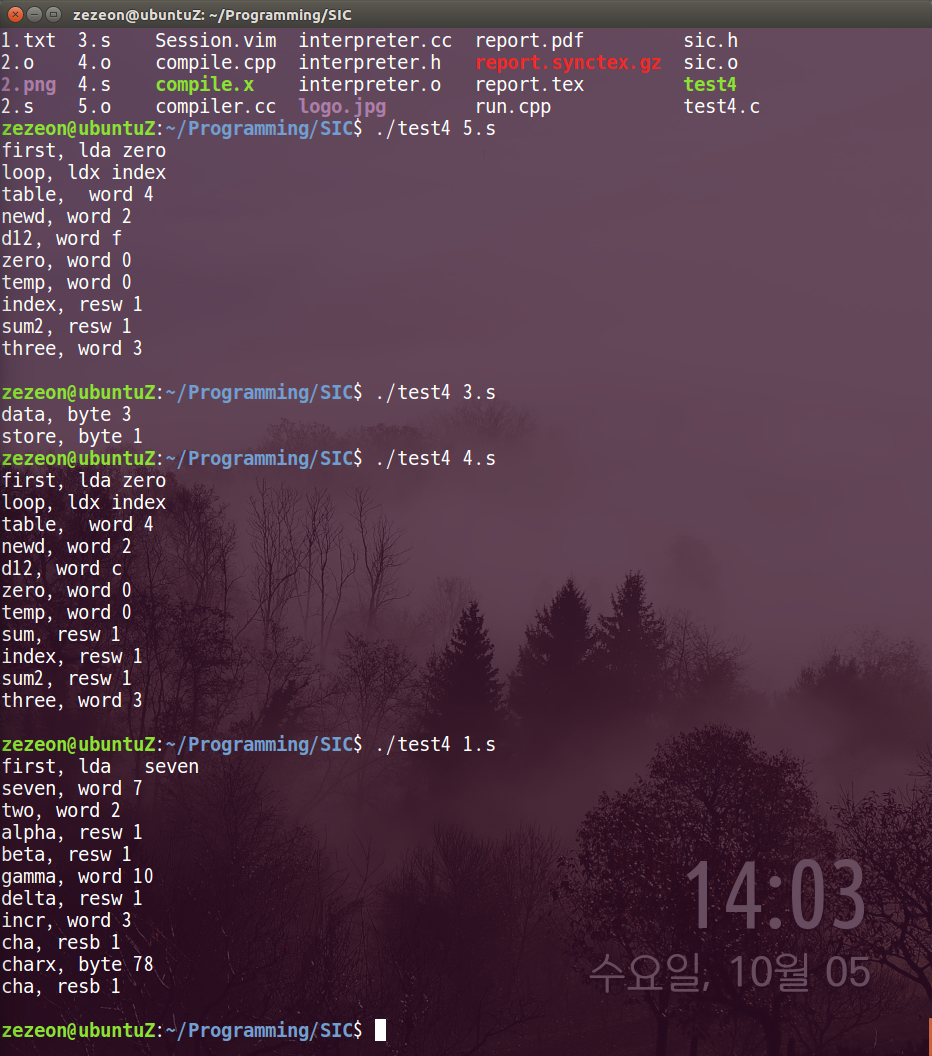
\includegraphics[width=\textwidth]{1.png}
\item 내장변수: \$\$(셸의 프로세스 id), \$0(셀 스크립트 이름), \$1...\$9(명령어 줄 인수 참조), \$*(모든 명령어 줄 인수의 목록), \$@(\$*의 변형)

\item 셀 스크립트 파일 작성
\lstinputlisting[caption={cat - \textgreater script.sh}]{script.sh}

\$chmod +x script.sh

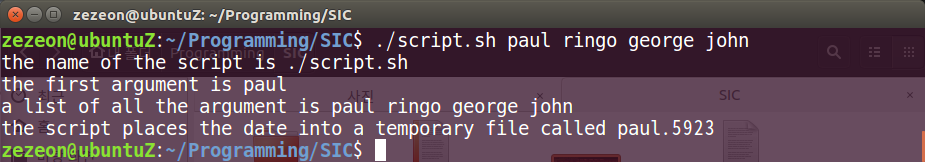
\includegraphics[width=\textwidth]{2.png}

\item .login file 보기

\lstinputlisting[caption={\$cat ~/.bashrc | more}]{/tmp/l}

\item 터미널 특성 변경 : stty\\
\$stty erase '\^H'\\
이미 터미널에 Ctrl-H가 셋팅되어 있었다.
\item 수행중인 프로세스 보기 : ps
\lstinputlisting[caption=출력결과]{/tmp/lll}
\item 지역변수 보기 : set\\
env로 실행시 환경변수를 볼 수 있었다.
\item 지역변수 설정 : set 변수명 = 변수값

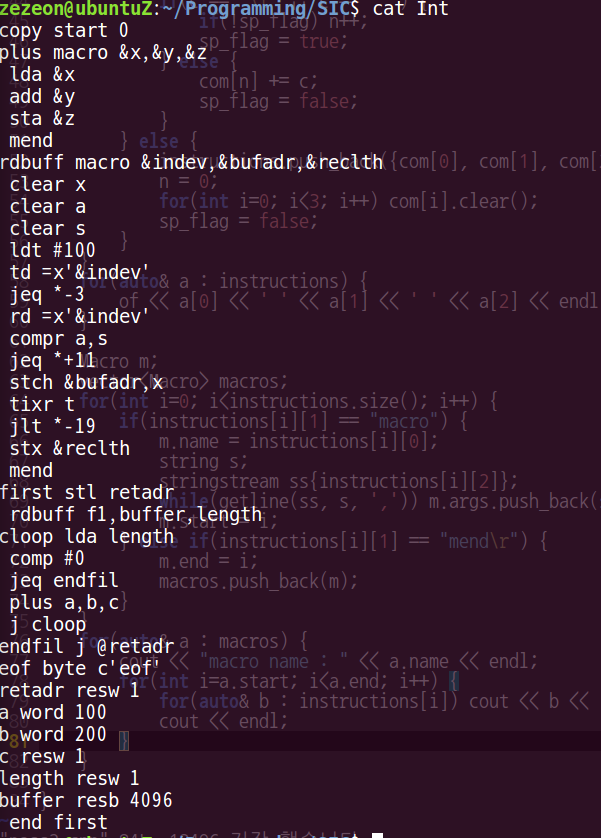
\includegraphics[width=\textwidth]{3.png}

\end{enumerate}

\item 다음과 같은 기능을 수행하는 script 파일 sample.sh을 생성하고 실행하시오.
\begin{enumerate}
	\item date 명령을 사용해서 현재 시간을 display 한다.
	\item who 명령을 사용해서 login 되어 있는 사용자 수를 display 한다.
	\item du -a 명령을 사용해서 disk file 크기를 display한다.
\end{enumerate}

\end{enumerate}
\lstinputlisting[caption=sample.sh]{sample.sh}
\lstinputlisting[caption=출력결과]{/tmp/ll}
{\Huge소감}
\indent
스크립트가 매우 유용하다는 것을 느꼈다.

\end{document}
